\documentclass{article}
\textheight24cm\textwidth16cm\topmargin-1cm
\oddsidemargin0cm\evensidemargin0cm

\usepackage{amsmath,amssymb}
% \usepackage[dvipdfmx]{graphicx}
\usepackage{graphicx}
\usepackage{subfigure}

\usepackage{url}
\usepackage{bm}
\usepackage{setspace} 
\usepackage{subfigure}

% \usepackage{algorithmic}
% \usepackage{algorithm}

\newtheorem{thm}{Theorem}
\newtheorem{dfn}[thm]{Definition}
\newtheorem{lem}[thm]{Lemma}
\newtheorem{prop}[thm]{Proposition}
\newtheorem{cor}[thm]{Corollary}
\newcommand{\proof}{\noindent Proof.\ \ }
% \renewcommand{\algorithmiccomment}[1]{// #1}


%\pagestyle{empty}


\begin{document}

% \baselineskip 6.5mm

\vspace*{1.0cm}
{\LARGE \bf Experiment on UCUT data with the various number of mutation signatures}
\vspace*{0.25cm}


We analyzed the data using our new model, with increasing number of mutation signatures $K=2,3,\dots$. 
Results are shown in Figure 1.
As expected, the likelihood increased with $K$. Bootstrap-errors started to increase at $K = 5$ (Figure 2).

With $K = 2$ (Figure 1(a)) we observed a mutation signature that appears to correspond to AA  (T $>$ A substitutions at CpTpG sites with strong transcription strand specificity).
Increasing to  $K=3$ introduced an additional mutation signature corresponding to the APOBEC enzyme (C $>$ [AGT] at TpCpN sites) (Figure 1(b)).
Increasing to $K = 4$ introduced an additional signature (T $>$ A at NpTpN sites with strong strand specificity) 
that is somewhat similar to the AA signature 
(Figure 1(c)). 
The membership in the AA signature and this ``AA-like" signature were correlated ($R = 0.77$; Figure 3). 
This additional signature may be just making up for the residual of the AA signature 
which the original AA signature could not explain due to a slight deviance of the probabilistic model.

The strong correlation among estimated membership parameters started to be shown at $K = 4$.
Considering all these factors together, $K = 3$ seems to be a reasonable choice in terms of the interpretability,
and we adopted $K = 3$.

\bibliographystyle{plain}
\bibliography{document}



\begin{figure}


\subfigure[$K = 2$]{%
  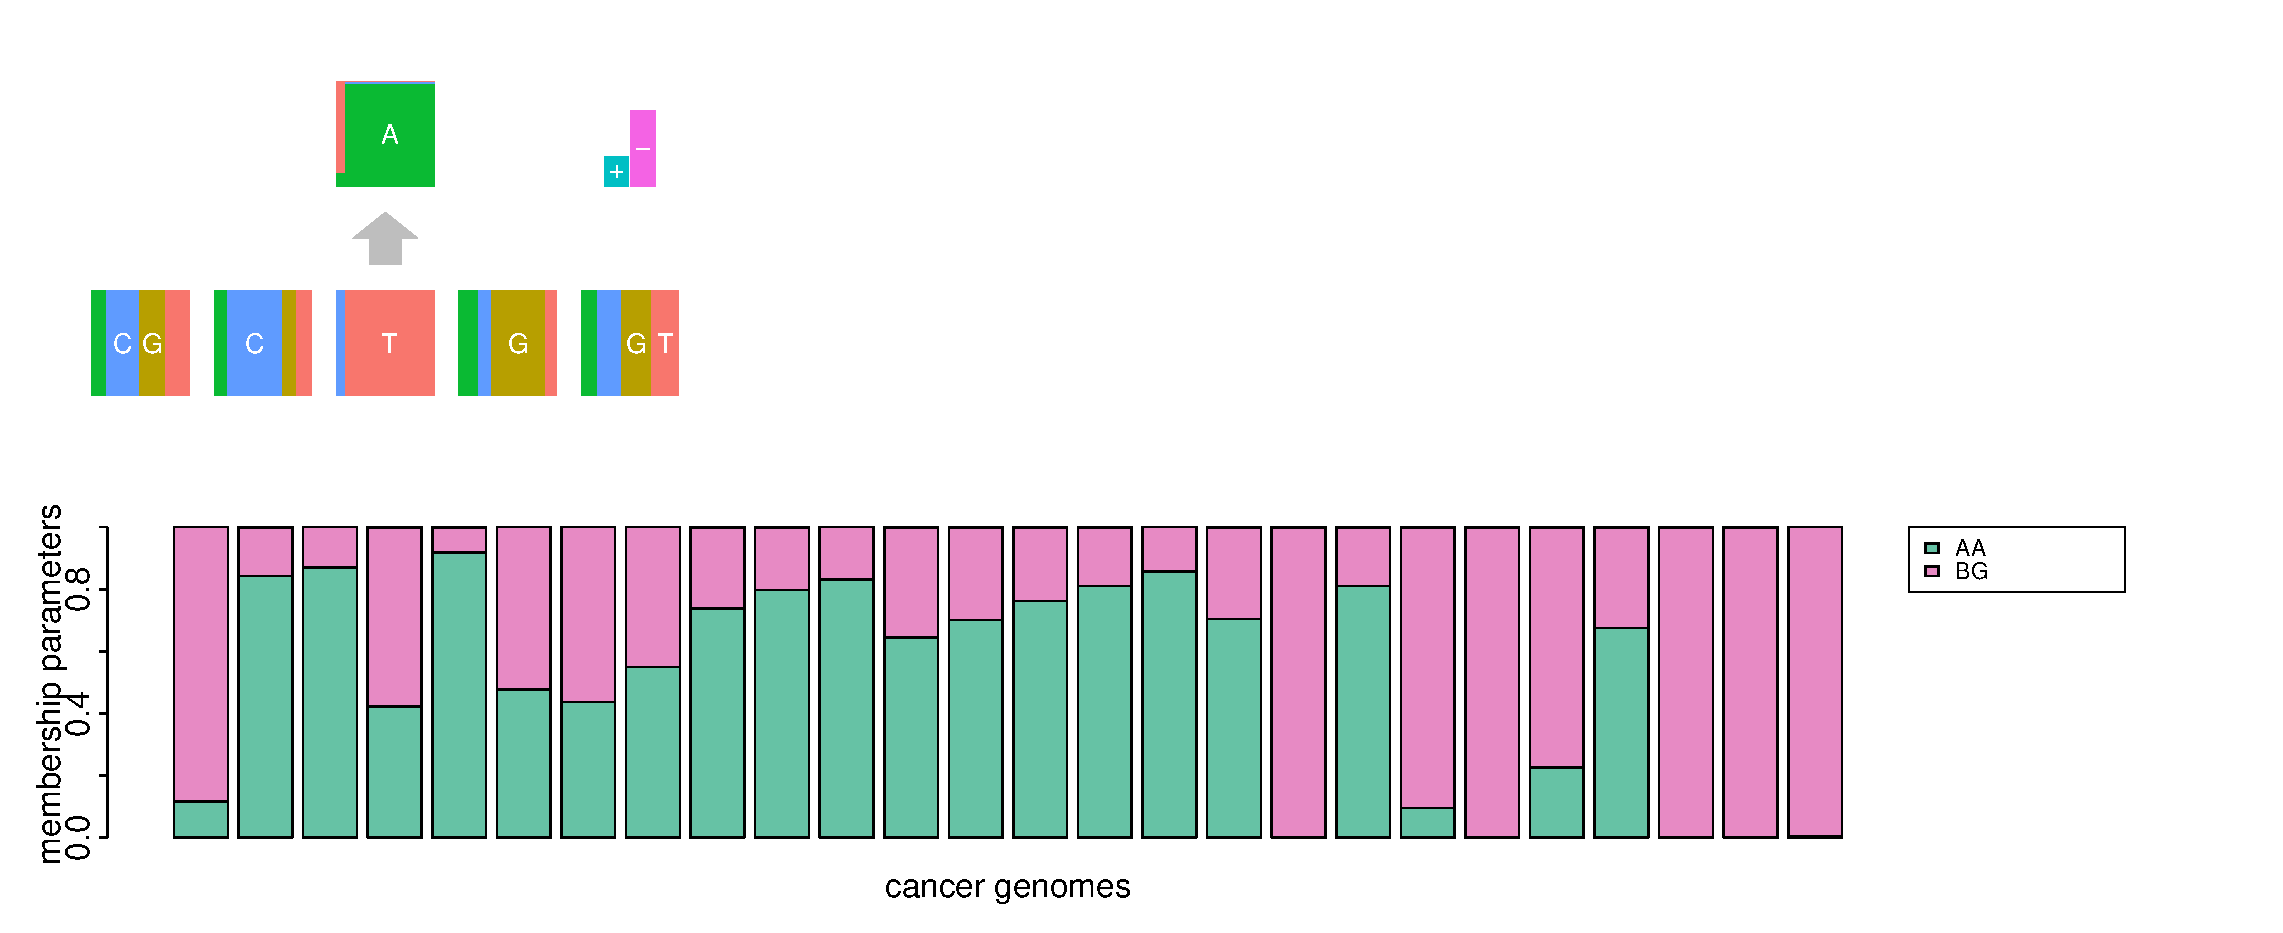
\includegraphics[height=6cm,width=15cm,clip]{UTUC_signature_K2.eps}
  \label{UTUC:sigK2_sig}}
  
  
\subfigure[$K = 3$]{%
  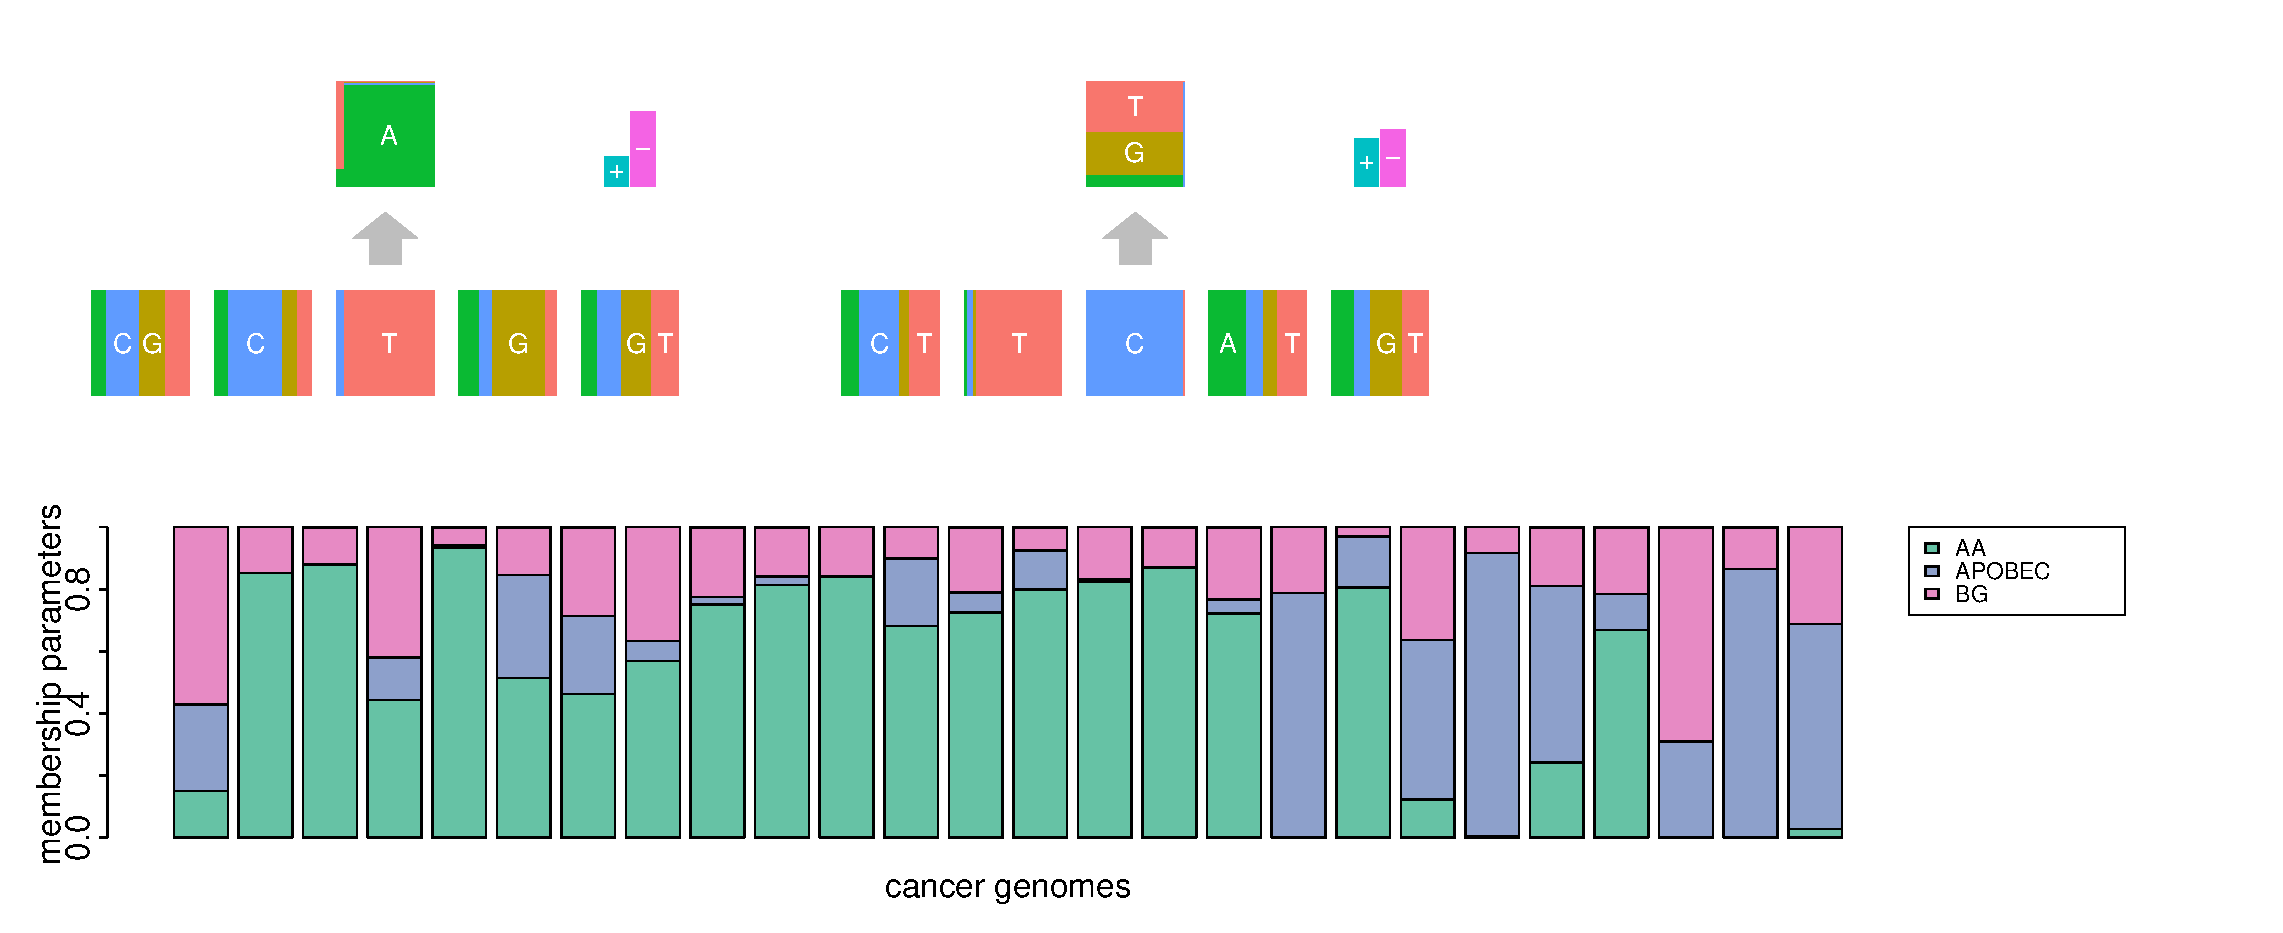
\includegraphics[height=6cm,width=15cm,clip]{UTUC_signature_K3.eps}
  \label{UTUC:sigK3_sig}}
  

\subfigure[$K = 4$]{%
  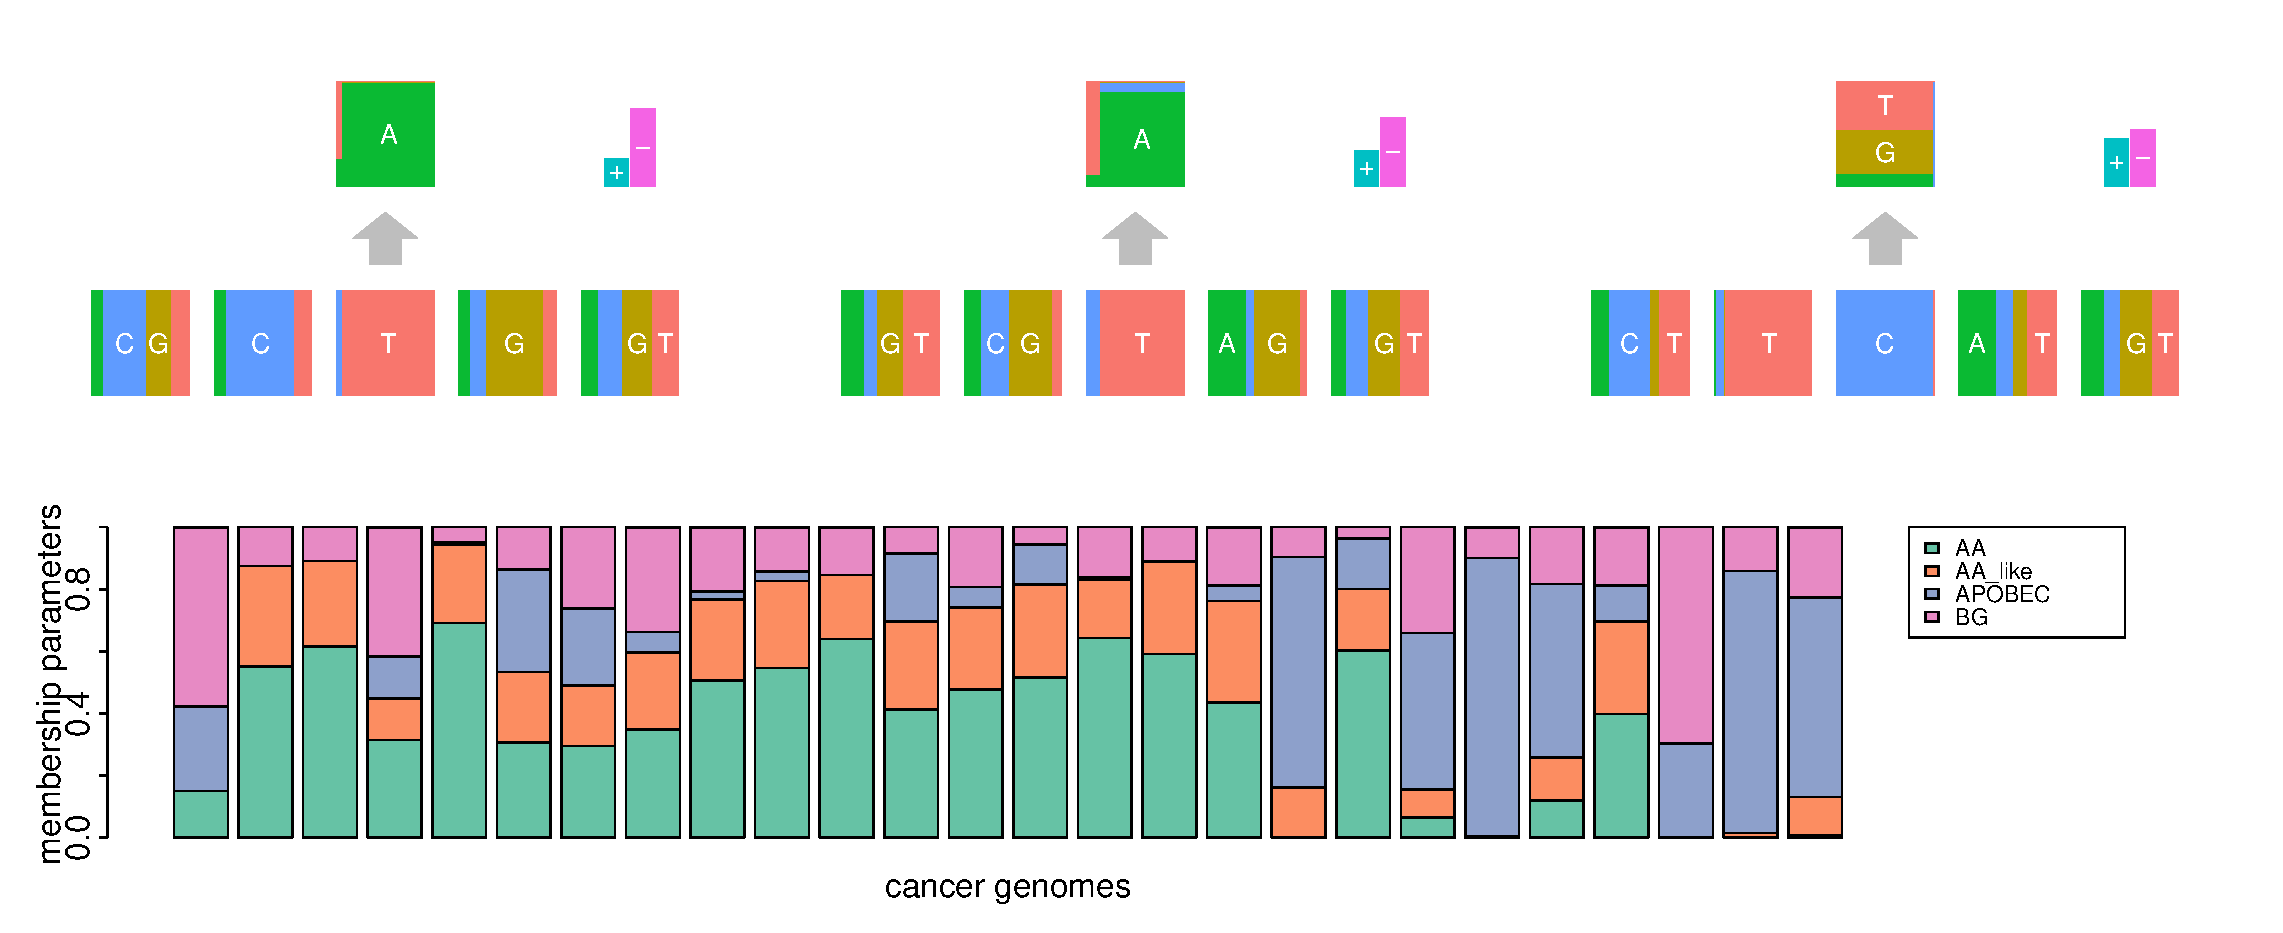
\includegraphics[height=6cm,width=15cm,clip]{UTUC_signature_K4.eps}
  \label{UTUC:sigK4_sig}}

  
\caption{The result of estimated mutation signatures and membership parameters for UTUC data 
when changing the number of mutation signatures $K$.}
\label{UTUC_multiK}
\end{figure}


\begin{figure}
\centering
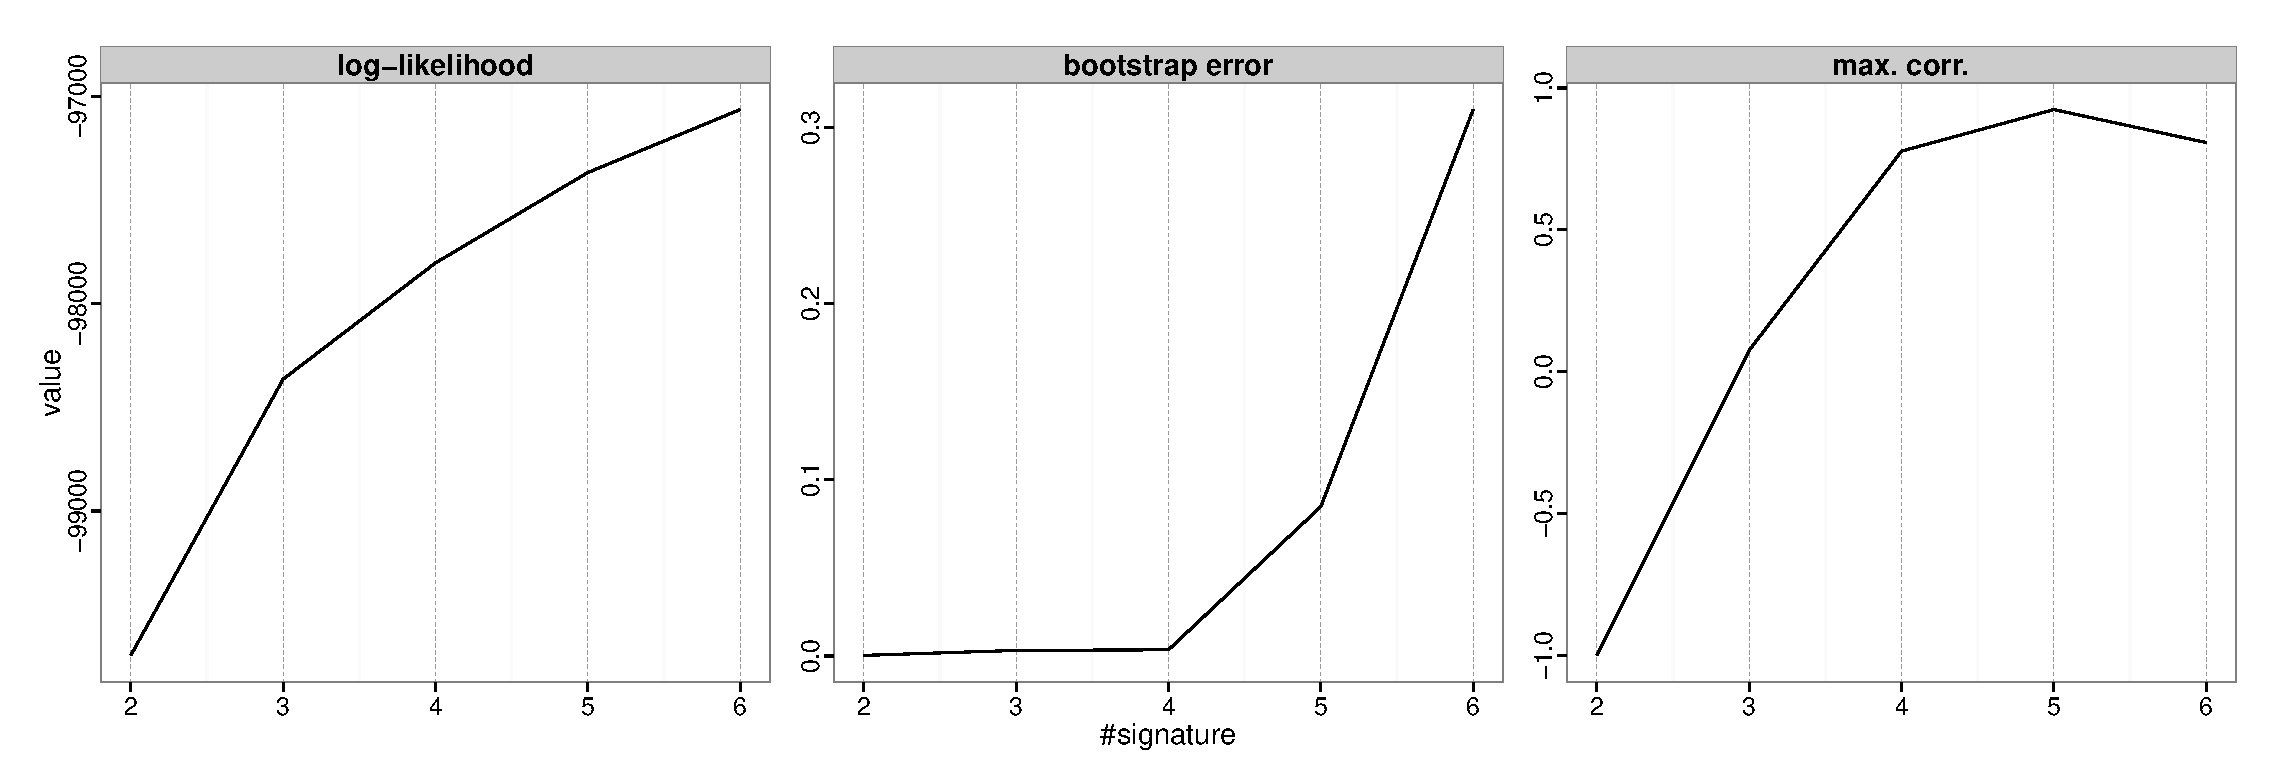
\includegraphics[width=15cm,height=5cm]{UTUC_stat.eps}
\caption{The log-likelihood, bootstrap-errors and maximum correlation values among estimated membership parameters for several numbers of signatures $K$ in UTUC data.}
\label{UTUC_stat}
\end{figure}


\begin{figure}
\centering
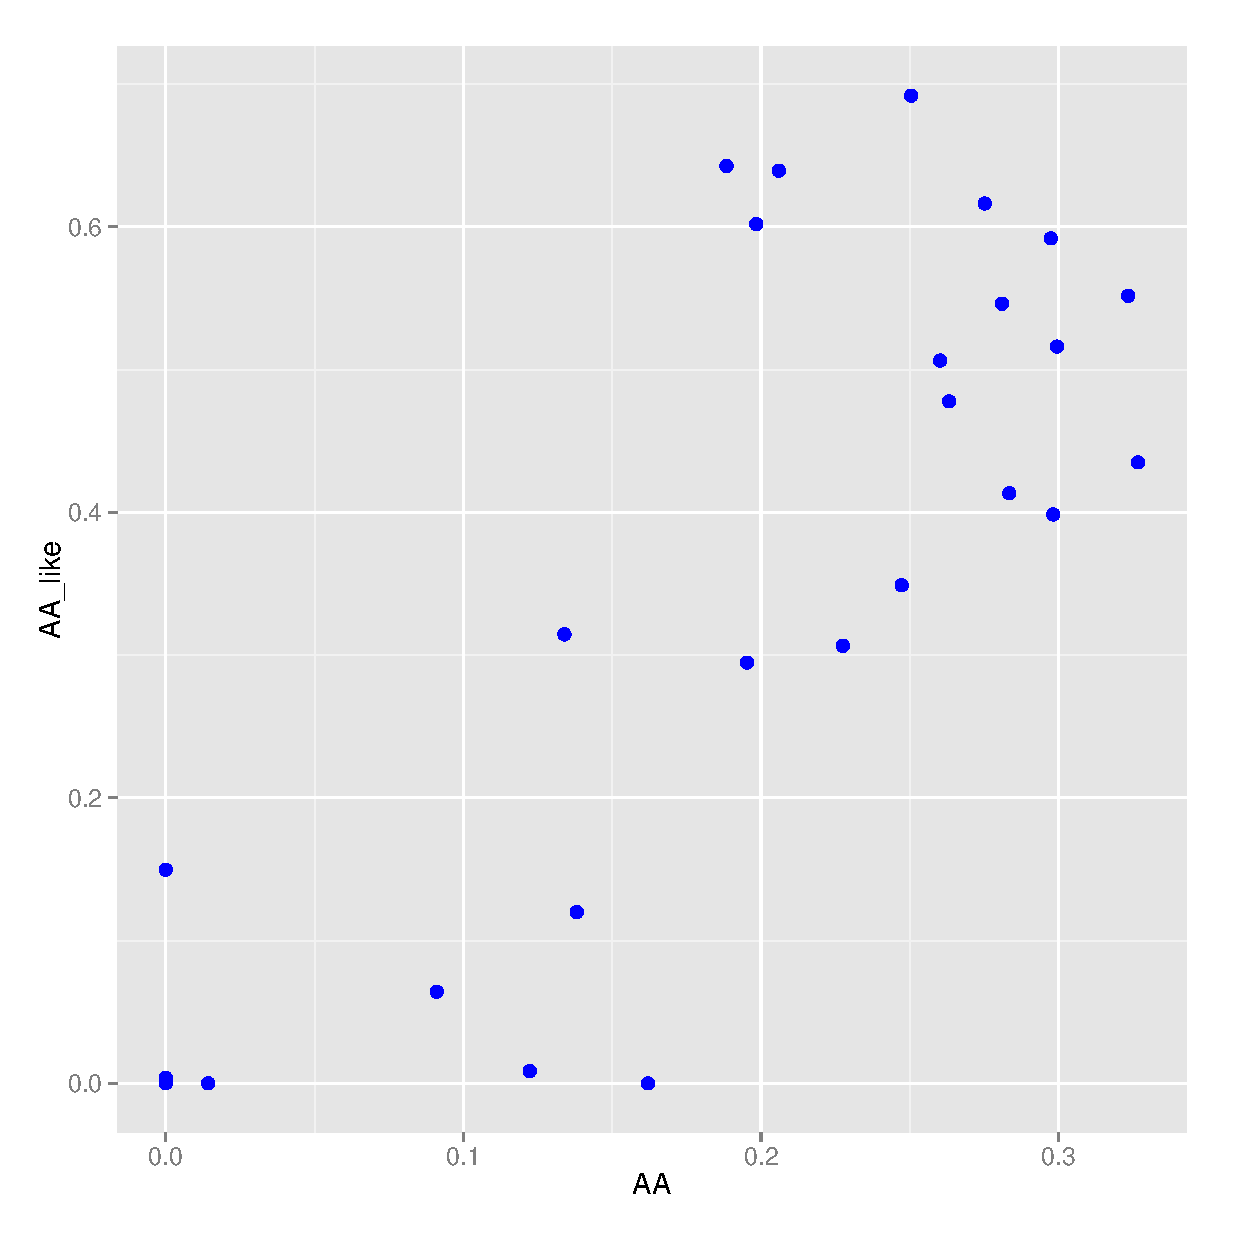
\includegraphics[width=10cm,height=10cm]{UTUC_AA_AAlike_cor.eps}
\caption{The relationships between the two membership parameters, AA (the first signature in the Figure 1(c)) and AA\_like (the second signature in the Figure 1(c)) signatures.}
\label{UTUT_AA_AAlike}
\end{figure}



\end{document}

